\documentclass[12pt,a4paper]{report}

% Packages
\usepackage[utf8]{inputenc}
\usepackage[english]{babel}
\usepackage{graphicx}
\usepackage{hyperref}
\usepackage{nomencl}
\usepackage{amsmath}
\usepackage{geometry}
\usepackage{setspace}
\usepackage{titlesec}
\usepackage{fancyhdr}
\usepackage{longtable}
\usepackage{listings}
\usepackage{xcolor}

% Page layout
\geometry{left=3cm, right=2cm, top=2.5cm, bottom=2.5cm}
\onehalfspacing

% Hyperref settings for clickable links
\hypersetup{
    colorlinks=true,
    linkcolor=black,
    filecolor=black,      
    urlcolor=black,
    citecolor=black,
    pdftitle={Airline Delay Analysis Database},
    pdfpagemode=FullScreen,
}

% List of Abbreviations
\makenomenclature

% Header and footer
\pagestyle{fancy}
\fancyhf{}
\renewcommand{\headrulewidth}{0pt}
\fancyfoot[C]{\thepage}

% Title formatting
\titleformat{\chapter}[display]
{\normalfont\huge\bfseries}{\chaptertitlename\ \thechapter}{20pt}{\Huge}
\titlespacing*{\chapter}{0pt}{-20pt}{40pt}

% Code listing settings
\lstset{
    basicstyle=\ttfamily\small,
    breaklines=true,
    frame=single,
    backgroundcolor=\color{gray!10},
}

\begin{document}

% Title Page
\begin{titlepage}
    \centering
    \vspace*{1cm}
    
    {\large MINISTRY OF EDUCATION AND TRAINING\par}
    {\large FPT UNIVERSITY\par}
    \vspace{2cm}
    
    {\LARGE\bfseries Airline Delay Analysis Database\par}
    \vspace{1.5cm}
    
    {\Large By\par}
    \vspace{1cm}
    
    {\large\bfseries GROUP 2\par}
    \vspace{0.5cm}
    {\large Dang Nguyen Minh An\par}
    {\large Pham Tuan Anh\par}
    {\large Nguyen Le Khiet\par}
    {\large Nguyen Minh Quang\par}
    {\large Dao Minh Tri\par}
    \vspace{2cm}
    
    {\large A thesis submitted in conformity with the requirements\par}
    {\large for the degree of Master of Software Engineering\par}
    \vspace{2cm}
    
    {\large © Copyright by Group 2 - 2026\par}
    
\end{titlepage}

% Table of Contents
\tableofcontents
\newpage

% List of Figures
\listoffigures
\addcontentsline{toc}{chapter}{List of Figures}
\newpage

% List of Tables
\listoftables
\addcontentsline{toc}{chapter}{List of Tables}
\newpage

% List of Abbreviations
\printnomenclature[4cm]
\addcontentsline{toc}{chapter}{List of Abbreviations}
\newpage

% Add abbreviations
\nomenclature{CSV}{Comma-Separated Values}
\nomenclature{HDFS}{Hadoop Distributed File System}
\nomenclature{API}{Application Programming Interface}
\nomenclature{SSE}{Server-Sent Events}
\nomenclature{SPA}{Single Page Application}
\nomenclature{UI}{User Interface}
\nomenclature{HTTP}{Hypertext Transfer Protocol}
\nomenclature{RAM}{Random Access Memory}
\nomenclature{ML}{Machine Learning}
\nomenclature{NAS}{National Airspace System}

% Abstract
\chapter*{Abstract}
\addcontentsline{toc}{chapter}{Abstract}

Airline delays are a persistent challenge in the aviation industry, affecting operational efficiency, airline costs, and passenger satisfaction. This report presents the design and analysis of an Airline Delay Analysis Database developed to explore patterns and factors contributing to flight delays using large-scale aviation data. Leveraging big data processing techniques, the system integrates and manages flight-related datasets containing information such as departure and arrival times, carrier details, airports, weather conditions, and delay causes.

The proposed database architecture enables efficient storage, querying, and analysis of high-volume flight data. Through data preprocessing, aggregation, and analytical queries, the study identifies common delay patterns across airlines, airports, and time periods. The analysis highlights key factors influencing delays, including carrier performance, airport congestion, and seasonal variations.

Additionally, the report demonstrates how big data technologies can support scalable data processing and facilitate meaningful insights from complex aviation datasets. The results provide valuable information for airlines, airport authorities, and researchers to better understand delay trends and potentially improve operational planning and decision-making.

Overall, this work illustrates the role of database design and big data analytics in transforming raw flight data into actionable knowledge for airline delay analysis.

\newpage

% Chapter 1: INTRODUCTION
\chapter{INTRODUCTION}

The objective of this chapter is to introduce the background and context of flight delay analysis in the airline industry. With the rapid growth of air transportation, flight delays have become a significant issue affecting both operational efficiency and passenger experience. This chapter begins by presenting an overview of the industry, the importance of the problem, and the motivation behind this study. It then defines the problem statement, highlighting the complexity of analyzing delays due to multiple influencing factors and large-scale heterogeneous data. Next, the scope and objectives of the study are outlined to clarify the research direction. Finally, a detailed description of the dataset, including its sources, key features, and challenges, is provided. Overall, this chapter establishes the foundation for applying data-driven approaches to analyze and predict flight delays.

\section{Airline Delay Background}

\subsection{Airline Industry Overview}

The airline industry plays a critical role in the global transportation system, enabling the movement of millions of passengers and goods every day. With the rapid growth in air travel demand, airlines operate a vast number of daily flights across complex networks of airports and routes.

However, managing such a large-scale system is highly challenging due to various operational, environmental, and logistical factors. Flight schedules must coordinate aircraft availability, crew assignments, airport capacity, and weather conditions, making the system inherently complex and dynamic.

Modern aviation systems generate massive amounts of data from multiple sources, including flight operations, airport information, weather conditions, and economic indicators. The integration of these heterogeneous data sources provides an opportunity to apply Big Data analytics and Machine Learning techniques to improve operational efficiency and decision-making.

\subsection{The Importance of the Problem}

Flight delays are one of the most significant challenges in the airline industry. They negatively impact passengers, airlines, and the overall transportation system. Delays can lead to passenger dissatisfaction, missed connections, and increased operational costs for airlines.

From an operational perspective, delays often propagate across the network, causing cascading effects on subsequent flights. Various factors contribute to flight delays, such as weather conditions, air traffic congestion, airline operations, and late aircraft arrivals.

The dataset used in this study integrates multiple data sources, including flight records, airport metadata, allowing for a comprehensive analysis of delay factors. Additionally, it contains detailed delay-related attributes such as carrier delay, weather delay, and late aircraft delay, which help identify the root causes of disruptions.

Therefore, understanding and predicting flight delays is essential for improving airline performance, optimizing resource allocation, and enhancing passenger experience.

\subsection{Motivation of our Study}

The motivation of this study arises from the increasing availability of large-scale aviation data and the need for data-driven decision-making in the airline industry. Traditional approaches to analyzing flight delays often rely on limited data and simple statistical methods, which may not fully capture the complexity of the problem.

With the availability of a large and rich dataset containing millions of flight records and multiple related data sources, it becomes possible to explore deeper insights into delay patterns and contributing factors. This dataset includes not only operational flight data but also external factors such as weather conditions and fuel prices, enabling a more holistic analysis.

The main motivation of this study is to leverage Big Data technologies and analytical methods to identify key factors influencing flight delays, and then analyze delay patterns across different airlines and airports, also support the development of predictive models for delay forecasting.

Ultimately, this study aims to contribute to improving airline operational efficiency and providing better decision support for stakeholders in the aviation industry.

\section{Problem Statement}

Despite the availability of large volumes of aviation data, accurately understanding and predicting flight delays remains a complex challenge. Flight delays are influenced by multiple interrelated factors, including weather conditions, airline operations, airport congestion, and aircraft scheduling. These factors often interact in non-linear and dynamic ways, making it difficult to identify the root causes using traditional analytical approaches.

In addition, the scale and heterogeneity of the data further complicate the problem. The dataset used in this study contains information from multiple sources, such as flight records, weather data, airport details, and economic indicators. Effectively integrating and analyzing such diverse data requires robust data processing and analytical techniques.

Therefore, the main problem addressed in this study is:

\begin{itemize}
    \item How to analyze large-scale flight data to identify key factors contributing to delays
    \item How to extract meaningful patterns from complex and high-dimensional data
    \item How to build reliable models to predict flight delays
\end{itemize}

Addressing these challenges is essential for improving decision-making and operational efficiency in the airline industry.

\section{Scope and Objectives}

This study aims to analyze and predict flight delays in the airline industry by leveraging large-scale aviation data and applying data-driven techniques. By integrating multiple data sources and utilizing analytical and machine learning approaches, the research seeks to uncover meaningful patterns and provide insights that can support decision-making and improve operational efficiency.

\subsection{Scope of the Study}

This study focuses on analyzing historical flight delay data using a large-scale dataset that integrates multiple sources, including flight operations, weather conditions, and airport information. The research emphasizes data preprocessing, feature engineering, and exploratory analysis within a Big Data context. Additionally, selected machine learning models are applied to predict flight delays. The study focuses on processing large-scale data. While the execution is batch-oriented, the system provides a real-time monitoring dashboard to visualize the pipeline progress and analytical results.

\subsection{Objectives}

The main objective of this study is to develop a data-driven approach for understanding and predicting flight delays. Specifically, the study aims to identify key factors influencing delays, analyze delay patterns across different conditions, and build predictive models to estimate delay occurrences. Furthermore, the research evaluates the performance of these models and provides insights that can contribute to improving airline operations and enhancing passenger experience.

\section{Data Description}

The dataset used in this study is provided on Hugging Face, named "flight\_delay", and is designed to support the analysis and prediction of flight delays in the United States aviation industry. This dataset integrates multiple heterogeneous data sources, enabling comprehensive exploration of factors influencing flight delays.

\begin{figure}[h]
    \centering
    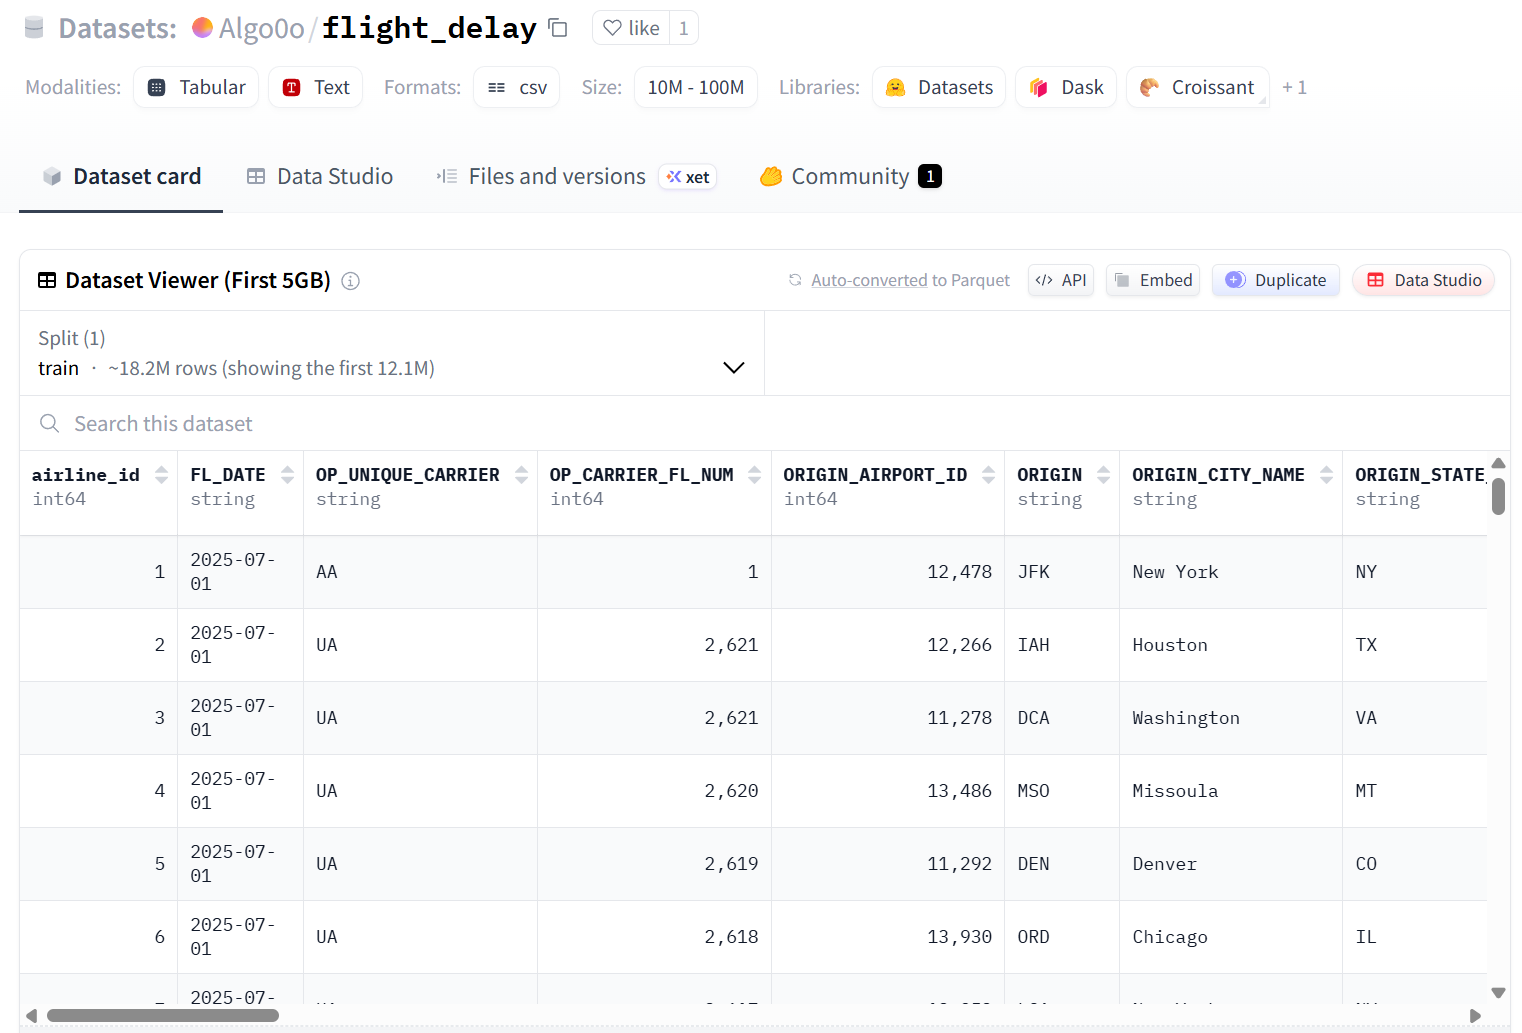
\includegraphics[width=0.9\textwidth]{figures/Bigdata_dataset.png}
    \caption{Flight Delay Dataset Overview and Structure}
    \label{fig:installation_workflow}
\end{figure}

\subsection{Dataset Overview}

\begin{itemize}
    \item \textbf{Name:} flight\_delay
    \item \textbf{Platform:} Hugging Face
    \item \textbf{Size:} Raw CSV data size: 3.4 GB (extracted from a 6.88 GB database package)
    \item \textbf{Scale:} Large-scale dataset with over 18 million flight records
    \item \textbf{Format:} CSV and SQLite database formats
    \item \textbf{Data Type:} Primarily tabular data (structured), including numerical and categorical features
\end{itemize}

This dataset was built to support analysis and prediction of flight delays in the US aviation industry by combining operational and external data sources.

\subsection{Database Structure and Tables}

The dataset is also provided as a SQLite database (airline\_delay\_analysis.db) consisting of multiple related tables:

\textbf{Airline:} Core table containing one record per flight. Includes detailed flight information such as departure/arrival time, delay status, and operational metrics.

\textbf{Airports:} Metadata about airports (location, codes, etc.)

\textbf{Carriers:} Information about airline companies

\textbf{Weather:} Daily weather data associated with flight locations

\textbf{FuelPrice:} Daily jet fuel price data

\textbf{FuelIndex:} Normalized fuel price index

\textbf{StockPrice:} Airline-related stock market data

These tables are interconnected, allowing multi-dimensional analysis of flight delays. This study primarily focuses on the Airline core table to analyze operational delays, while other tables provide potential for future extended analysis.

\subsection{Key Features}

The Airline table (main table) includes a wide range of attributes such as:

\begin{itemize}
    \item \textbf{Flight information:} flight date, carrier, flight number
    \item \textbf{Location data:} origin and destination airports
    \item \textbf{Time-related variables:} scheduled and actual departure/arrival times
    \item \textbf{Delay metrics:}
    \begin{itemize}
        \item Departure delay (DEP\_DELAY)
        \item Arrival delay (ARR\_DELAY)
        \item Delay categories (carrier, weather, NAS, late aircraft)
    \end{itemize}
    \item \textbf{Operational indicators:} cancellation, diversion, elapsed time, distance
\end{itemize}

These features enable both descriptive analysis and predictive modeling of delays.

\subsection{Data Processing Objectives}

\begin{figure}[h]
    \centering
    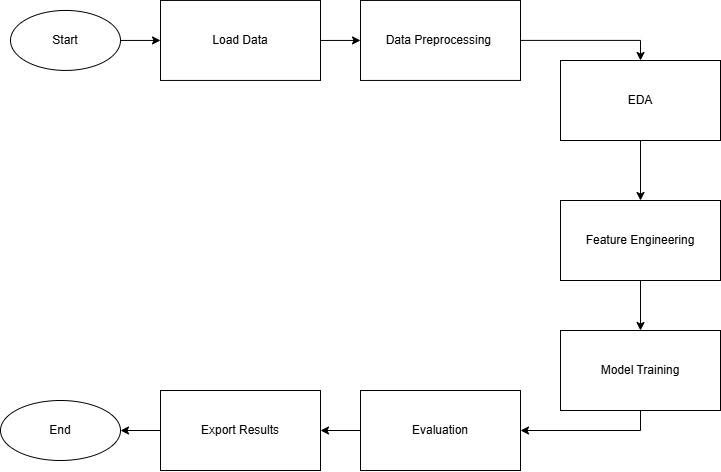
\includegraphics[width=0.9\textwidth]{figures/Bigdata_DataProcessingObject.jpg}
    \caption{Data Processing Pipeline Objectives and Workflow}
    \label{fig:installation_workflow}
\end{figure}

The data processing pipeline in this study is designed to efficiently handle large-scale flight delay data and transform it into a structured format suitable for analysis and prediction. The primary objective is to ensure data quality, reduce computational overhead, and enable scalable analytics using distributed processing with Apache Spark.

First, the pipeline aims to perform efficient data ingestion from distributed storage (HDFS) with fallback to local storage when necessary. To optimize I/O performance, only essential columns are selected through column pruning, reducing unnecessary data loading and improving processing efficiency.

Second, the pipeline focuses on data cleaning and preprocessing to ensure data reliability and consistency. This process includes filtering out cancelled flights, removing irrelevant or redundant columns, and handling missing values by dropping records with critical null fields (such as delay and location attributes). For delay-related features, missing values are imputed with default values (e.g., zero). Additionally, data type standardization is performed by casting key attributes (such as delay and distance) into appropriate numerical formats. These steps help eliminate noise, reduce data inconsistency, and prepare the dataset for accurate analysis.

Third, the pipeline supports descriptive analytics and aggregation, enabling the extraction of meaningful insights from large-scale data. This includes analyzing delay causes, identifying airports with high delay rates, and examining temporal delay trends. These insights help uncover patterns and key factors influencing flight delays.

Finally, the pipeline aims to facilitate machine learning-based prediction by preparing a structured dataset for modeling. This involves feature engineering, encoding categorical variables, constructing feature vectors, and training a classification model (Decision Tree) to predict flight delays. The model is evaluated using accuracy metrics, and feature importance is analyzed to interpret the impact of different variables.

Overall, the data processing objectives are to build a scalable, efficient, and end-to-end pipeline that transforms raw flight data into actionable insights and predictive models for flight delay analysis.

% Chapter 2: SYSTEM ARCHITECTURE OVERVIEW
\chapter{SYSTEM ARCHITECTURE \\ OVERVIEW}

\section{System Overview}

\subsection{Purpose}

The system is built with the purpose of creating a large-scale flight data analysis platform capable of processing over 18 million flight records. This platform not only performs in-depth analysis of the causes leading to flight delays but also integrates Machine Learning algorithms, specifically Decision Tree, to predict the probability of future flight delays. All analysis results are displayed in real-time on a web dashboard, allowing users to monitor and evaluate data in an intuitive and efficient manner.

\subsection{System Architecture Diagram}

\begin{figure}[h]
    \centering
    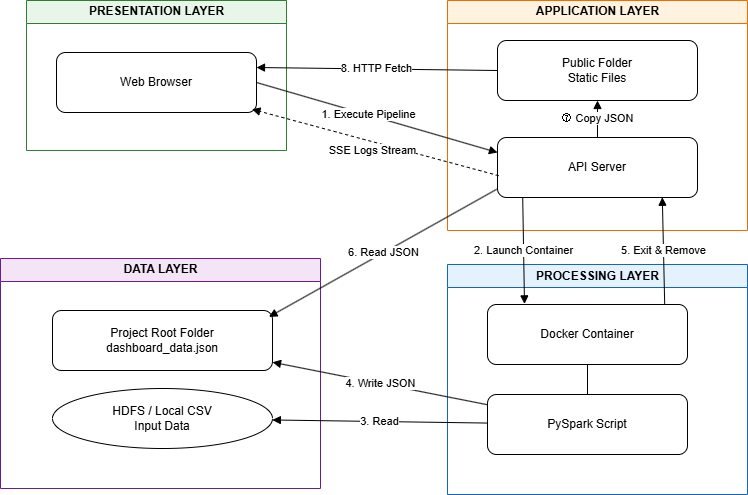
\includegraphics[width=0.9\textwidth]{figures/Bigdata_SystemOverview.drawio.png}
    \caption{System Architecture Diagram}
    \label{fig:system_architecture}
\end{figure}

\subsection{System Workflow Description}

The system operates through a streamlined architecture with clear separation of concerns. The flow begins when the user accesses the web dashboard and clicks the "Execute Pipeline" button. The browser establishes an EventSource connection to \texttt{/api/run}, enabling real-time bidirectional communication.

The API Server receives the request and spawns a Docker container with the command: \texttt{docker run --rm --network hadoop-docker\_default -v "\$\{projectRoot\}:/app" -w /app my\_pyspark\_edge python final\_project.py}. The \texttt{--rm} flag ensures the container auto-removes after execution. The volume mount \texttt{-v "\$\{projectRoot\}:/app"} creates a bridge where the project root directory on the host is accessible as \texttt{/app} inside the container.

Inside the container, the PySpark script executes four processing phases: Data Ingestion, Cleaning, Analysis, and Machine Learning. The script reads input data from either HDFS cluster (primary) or local CSV file (fallback). After processing completes, the script writes results to \texttt{dashboard\_data.json} in the working directory \texttt{/app}, which physically exists in \texttt{projectRoot} on the host machine due to the volume mount.

Once processing finishes, the container exits and Docker automatically removes it. The API Server detects the exit event and copies the JSON file from \texttt{projectRoot/dashboard\_data.json} to \texttt{dashboard/public/dashboard\_data.json}, making it accessible as a static file. The Frontend then fetches this file via HTTP request and renders the analytical charts. Throughout execution, the API streams real-time logs to the browser via Server-Sent Events (SSE).

The volume mount mechanism enables seamless data flow between the isolated container and host system, supporting the stateless container pattern where containers can be destroyed after execution while preserving their output.

\section{Deployment Architecture}

\subsection{Multi-Layer Architecture Diagram}

\begin{figure}[h]
    \centering
    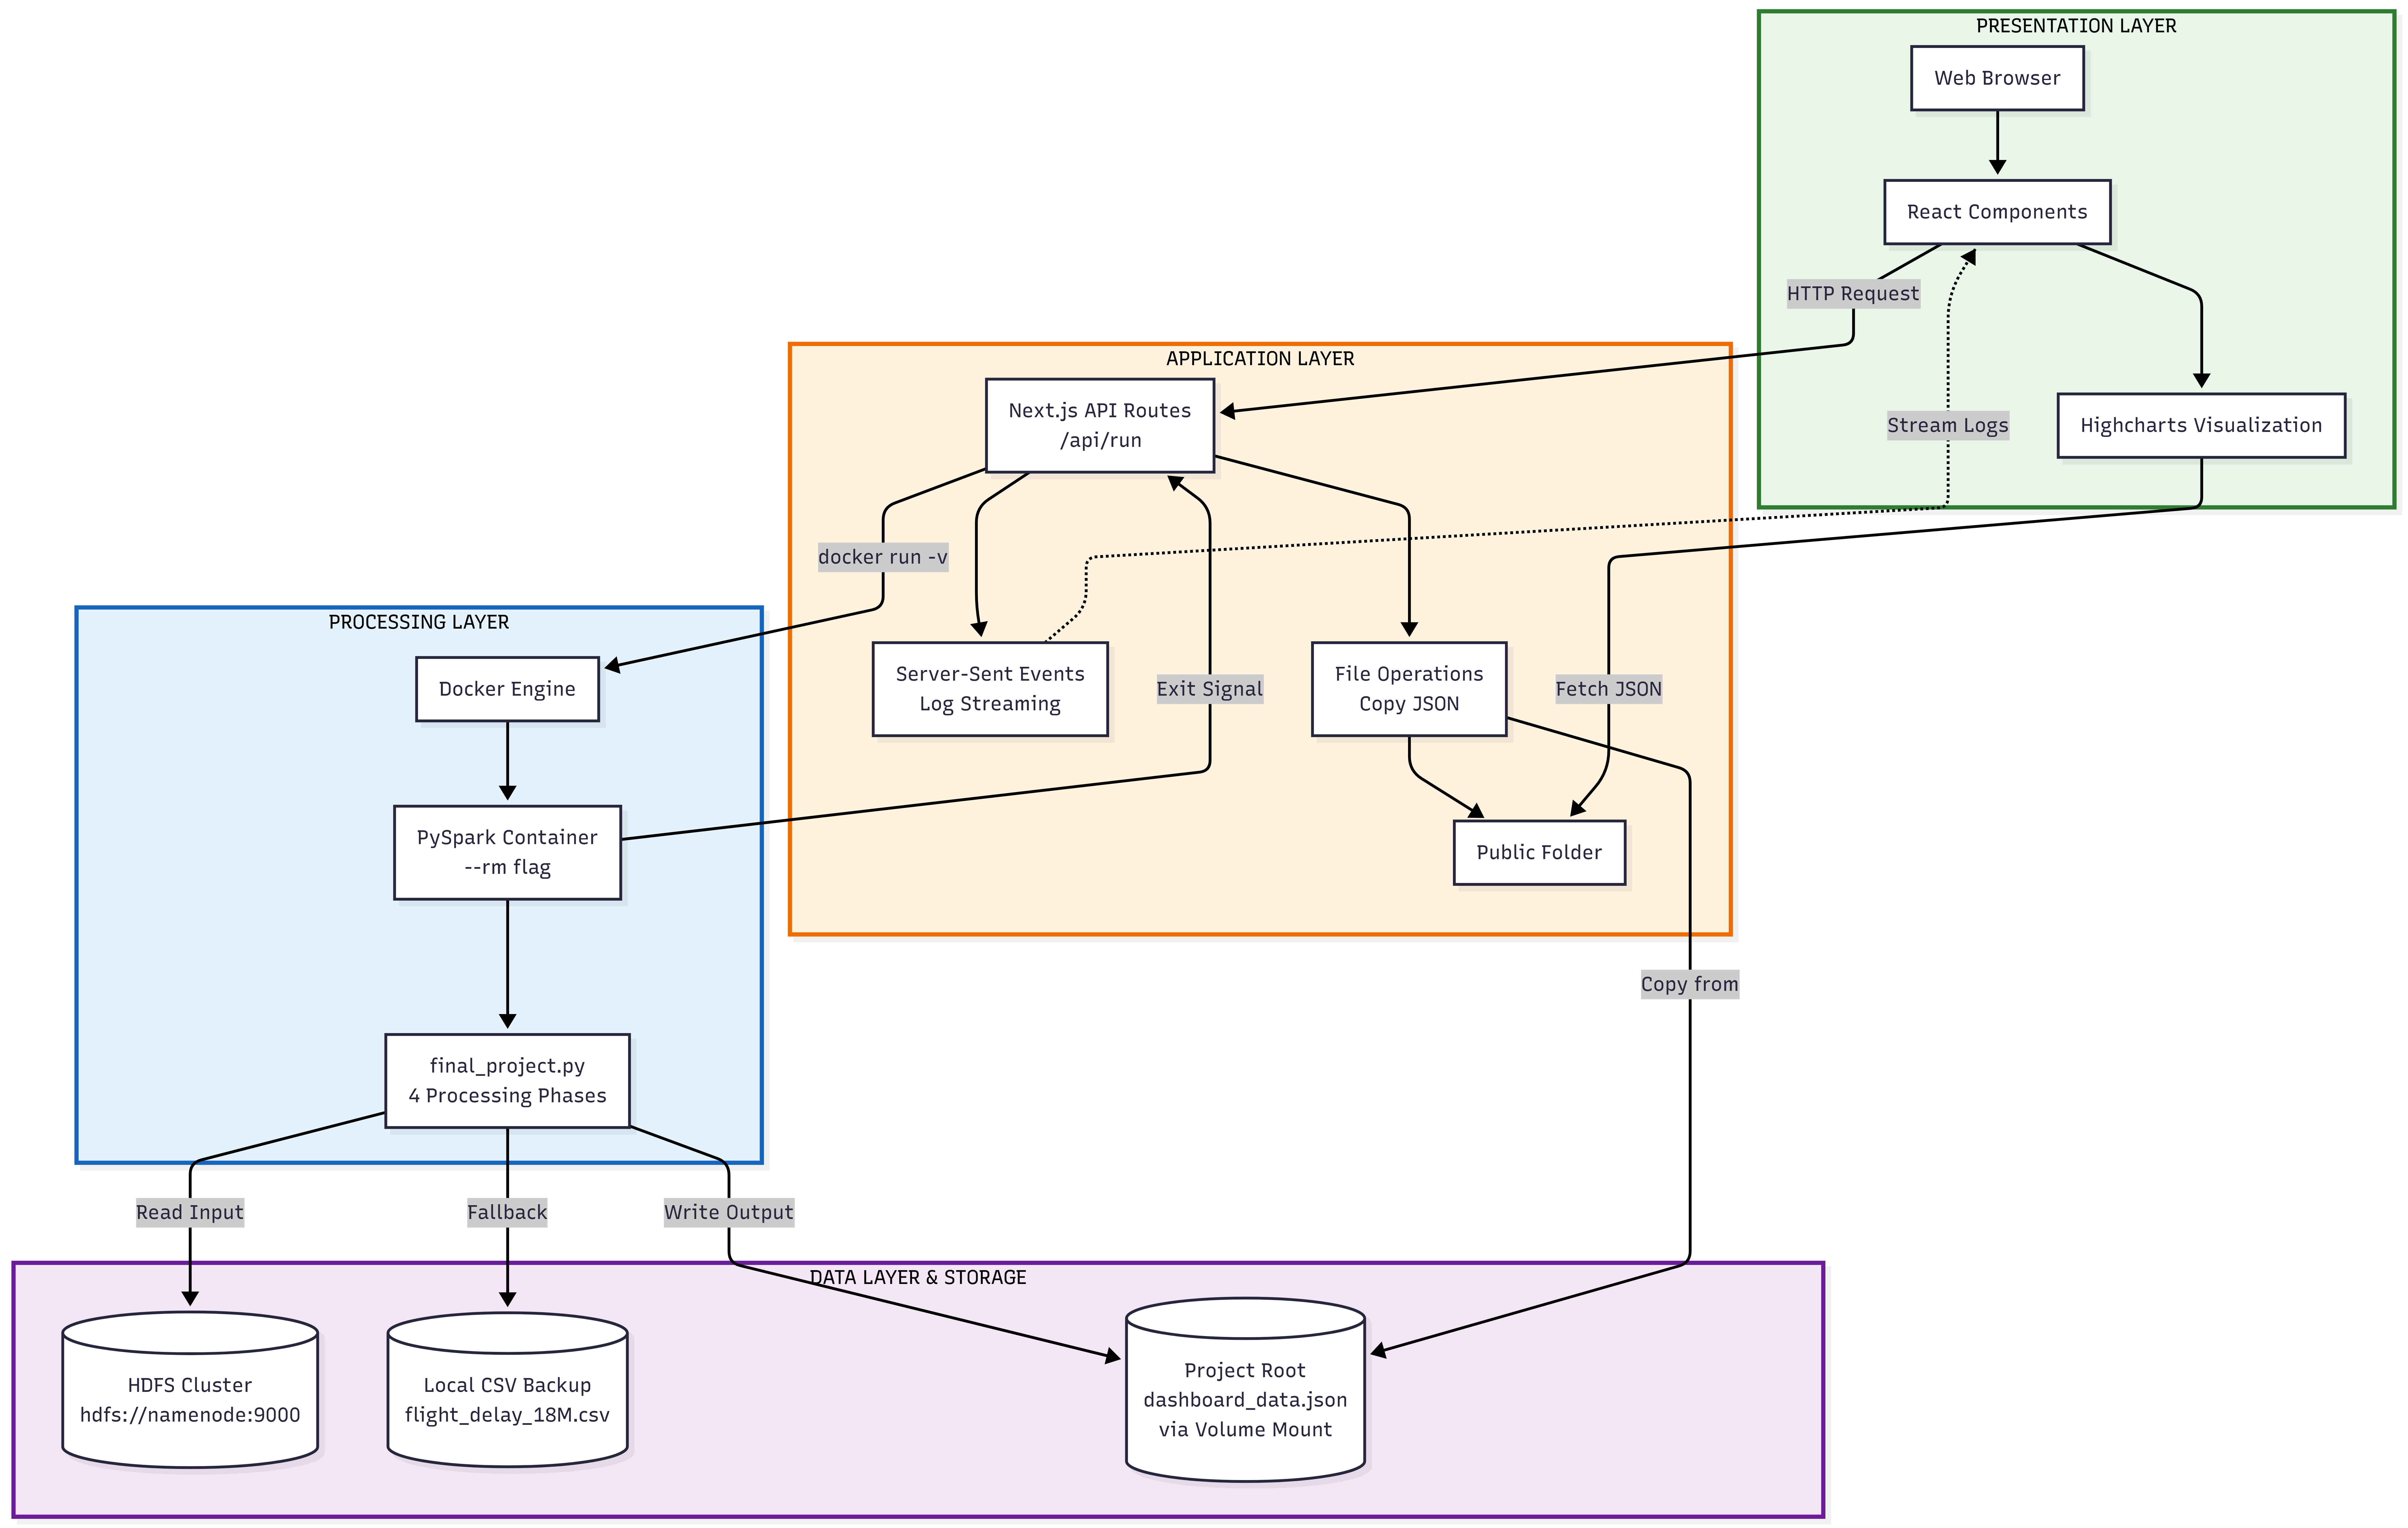
\includegraphics[width=0.9\textwidth]{figures/Bigdata_LayerSystem.png}
    \caption{Multi-Layer Architecture Diagram}
    \label{fig:deployment_architecture}
\end{figure}

\subsection{Layer Descriptions}

\subsubsection{Layer 1 - Presentation}

The Presentation layer serves as the user-facing interface built on Next.js and React. The Web Browser hosts the Single Page Application (SPA) that renders the interactive dashboard. React Components manage the UI state and user interactions, utilizing Ant Design for consistent UI elements. Highcharts Visualization library is integrated to render complex analytical charts including pie charts for delay causes, column charts for airport rankings, and line charts for monthly trends. This layer communicates with the backend via EventSource for real-time log streaming and standard HTTP requests for fetching static JSON files.

\subsubsection{Layer 2 - Application}

The Application layer orchestrates the entire pipeline execution and data flow management. The Next.js API Routes (\texttt{/api/run}) handle incoming pipeline execution requests and spawn Docker containers. Server-Sent Events (SSE) provides a unidirectional channel to stream real-time processing logs from the container stdout/stderr to the browser, enabling users to monitor progress. File Operations component manages the critical task of copying the generated JSON file from the project root (where the container writes via volume mount) to the public folder for static file serving. This layer acts as the bridge between the stateless frontend and the ephemeral container backend.

\subsubsection{Layer 3 - Processing}

The Processing layer executes the Big Data analytics workload in an isolated containerized environment. Docker Engine manages the container lifecycle, spawning containers on-demand with the \texttt{--rm} flag for automatic cleanup after execution. The PySpark Container runs on the custom image \texttt{my\_pyspark\_edge}, which includes Python, OpenJDK, and PySpark dependencies. Inside the container, \texttt{final\_project.py} executes four sequential processing phases: Data Ingestion (reading 18M records), Data Cleaning (filtering and type casting), Data Analysis (aggregations and rankings), and Machine Learning (Decision Tree classifier training). The container operates with a volume mount, allowing it to write output files that persist on the host machine even after the container is removed.

\subsubsection{Layer 4 - Data Layer \& Storage}

The Data layer manages all data persistence and retrieval operations. HDFS Cluster serves as the primary distributed storage system, providing scalability and fault tolerance for the 3.4GB input dataset. Local CSV Backup (\texttt{flight\_delay\_18M.csv}) acts as a fallback data source when HDFS is unavailable, ensuring system resilience. Project Root functions as the output destination where \texttt{dashboard\_data.json} is written via volume mount. The volume mount mechanism (\texttt{-v "\$\{projectRoot\}:/app"}) creates a transparent bridge where files written to \texttt{/app} inside the container appear in the project root on the host. This architecture enables the stateless ephemeral container pattern while preserving output data across container lifecycles.

\section{System Execution Flow}

\subsection{Sequence Diagram}

\begin{figure}[h]
    \centering
    \includegraphics[width=0.9\textwidth]{figures/Bigdata_SequenceDiagram.png}
    \caption{System Execution Flow Sequence Diagram}
    \label{fig:sequence_diagram}
\end{figure}

\subsection{Execution Flow Description}

The system execution flow is initiated by the user through the web browser interface. Upon receiving this request, the Next.js API immediately spawns a Docker container containing the PySpark environment to handle the request. The PySpark container then proceeds to execute four data processing phases in a sequential and systematic manner.

Throughout the processing, intermediate and final results are written to a JSON file, while the system simultaneously streams real-time logs to the Frontend, allowing users to monitor the processing progress. This creates a good interactive experience and helps users stay informed about the system's processing status. When the processing is complete, the dashboard automatically fetches the JSON file containing the results and displays the analytical charts in an intuitive and comprehensible manner for the user.

% Chapter 3: TECHNOLOGIES USED & INSTALLATION GUIDE
\chapter{TECHNOLOGIES USED \& \\ INSTALLATION GUIDE}

\section{Technologies Used}

\subsection{Technology Overview}

\begin{table}[h]
    \centering
    \label{tab:technologies}
    \begin{tabular}{|l|l|p{7cm}|}
        \hline
        \textbf{Category} & \textbf{Technology} & \textbf{Purpose} \\
        \hline
        Big Data Processing & Apache Spark & Distributed data processing for 18M+ records \\
        \hline
        Container Platform & Docker & Isolated execution environment \\
        \hline
        Frontend Framework & Next.js & Full-stack web application framework \\
        \hline
        UI Library & React & Interactive user interface components \\
        \hline
        UI Components & Ant Design & Professional UI component library \\
        \hline
        Visualization & Highcharts & Interactive data visualization charts \\
        \hline
        Programming Language & Python & Data processing and ML implementation \\
        \hline
        ML Library & Spark MLlib & Machine learning model training \\
        \hline
        Distributed Storage & HDFS & Hadoop Distributed File System \\
        \hline
    \end{tabular}
    \caption{Technologies and Tools Used in the System}
\end{table}

\subsection{Why Apache Spark?}

Apache Spark was chosen as the core data processing engine for several compelling reasons:

\begin{itemize}
    \item \textbf{Performance:} Successfully processes 18 million records in approximately 142 seconds, while Pandas fails due to memory limitations
    \item \textbf{In-Memory Computing:} Uses in-memory computing, significantly improving performance (10--100$\times$ faster than Hadoop MapReduce in many cases)
    \item \textbf{Comprehensive Components:} Provides built-in components:
    \begin{itemize}
        \item Spark SQL for data querying
        \item MLlib for machine learning tasks
    \end{itemize}
    \item \textbf{Easy Deployment:} Easy deployment on distributed environments or via containers (Docker)
\end{itemize}

\subsection{Why Next.js?}

Next.js was selected as the web application framework due to its advantages:

\begin{itemize}
    \item \textbf{Full-Stack Architecture:} Supports a full-stack architecture (frontend and backend in a single project)
    \item \textbf{Built-in API Routes:} Built-in API routes, eliminating the need for a separate backend server
    \item \textbf{Performance Optimization:} Performance optimization features:
    \begin{itemize}
        \item Server-Side Rendering (SSR)
        \item Static Site Generation (SSG)
    \end{itemize}
    \item \textbf{Dashboard Support:} Well-suited for building interactive data dashboards
\end{itemize}

\section{System Setup and Execution Workflow}

The system deployment process consists of the following main steps:

\begin{enumerate}
    \item Install required tools (Docker, Node.js, Python, Java)
    \item Clone the project repository
    \item Download the dataset (approximately 3.4GB)
    \item Build the Docker image containing the Spark environment
    \item Install the frontend dashboard dependencies
    \item Start the dashboard application
    \item Execute the data processing pipeline
\end{enumerate}

After setup:
\begin{itemize}
    \item Users can trigger the pipeline through the web interface
    \item Results are displayed as interactive charts on the dashboard
\end{itemize}

% Chapter 4: MAIN SOURCE CODE AND ANALYSIS RESULT
\chapter{MAIN SOURCE CODE AND \\ ANALYSIS RESULTS}

This chapter presents the implementation details and analytical results obtained from processing the 18-million-record flight delay dataset. The analysis pipeline successfully executed four sequential phases: Data Ingestion, Data Cleaning, Data Analysis, and Machine Learning, producing comprehensive insights into flight delay patterns and predictive capabilities.

\section{Pipeline Execution Overview}

The data processing pipeline was executed using Apache Spark within a Docker containerized environment. The system processed the entire dataset through distributed computing, applying column pruning and optimized partitioning strategies to enhance performance. The pipeline completed in approximately 133 seconds, demonstrating efficient handling of large-scale data.

\subsection{Processing Phases Summary}

\begin{itemize}
    \item \textbf{Phase 1 - Data Ingestion:} Successfully loaded 18.2 million flight records from HDFS/local storage with selective column loading
    \item \textbf{Phase 2 - Data Cleaning:} Filtered cancelled flights, handled missing values, and standardized data types, resulting in 17.5 million valid records
    \item \textbf{Phase 3 - Data Analysis:} Performed aggregations to identify delay causes, worst-performing airports, and temporal patterns
    \item \textbf{Phase 4 - Machine Learning:} Trained a Decision Tree classifier achieving 79.46\% accuracy for delay prediction
\end{itemize}

\section{Machine Learning Results and Key Metrics}

\begin{figure}[h]
    \centering
    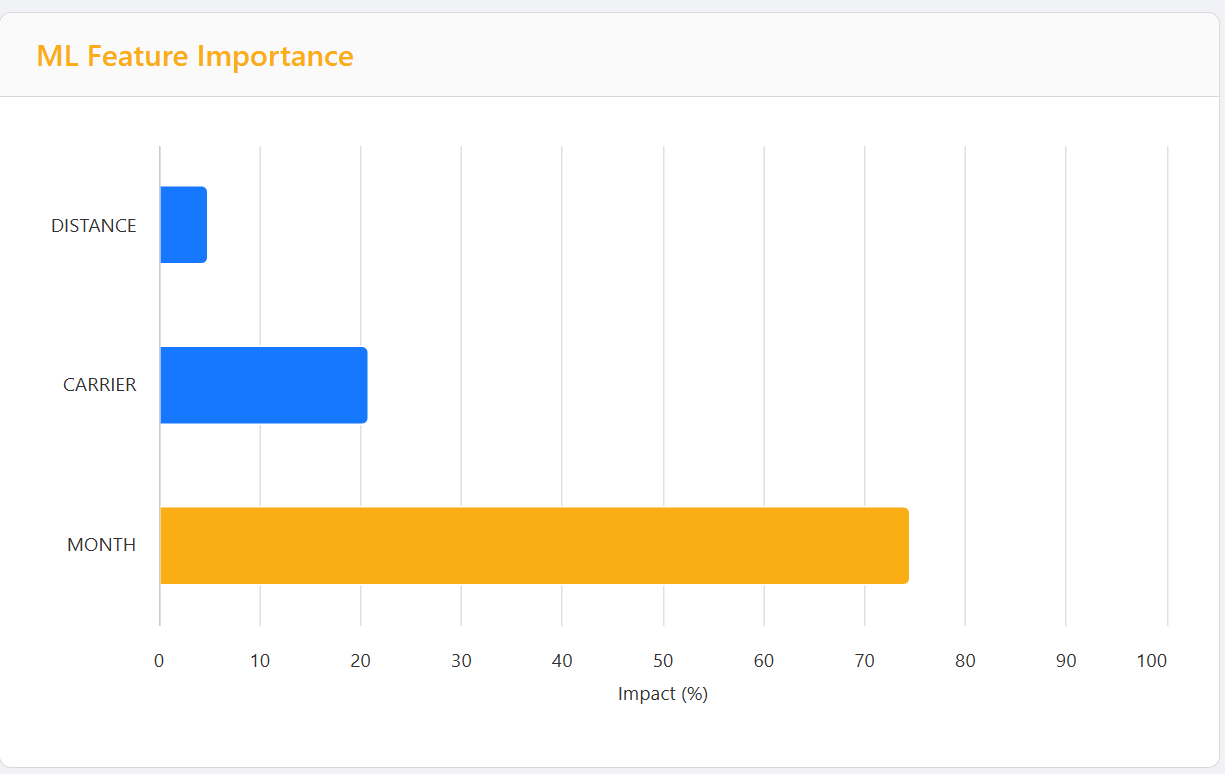
\includegraphics[width=0.9\textwidth]{figures/Bigdata_MLResults_KeyMetrics.png}
    \caption{Machine Learning Accuracy and Key Performance Metrics}
    \label{fig:ml_results}
\end{figure}

The machine learning model delivered significant predictive performance, achieving an accuracy of 79.46\% in classifying flight delays. This result demonstrates that the selected features (carrier, distance, and month) provide substantial predictive power for delay forecasting.

\subsection{Key Findings}

\textbf{ML Accuracy:} The Decision Tree classifier achieved 79.46\% accuracy on the test dataset, indicating that approximately 4 out of 5 flight delay predictions are correct. This performance level is suitable for operational decision support and preliminary screening of high-risk flights.

\textbf{Worst Delay Airport:} Fort Lauderdale-Hollywood International Airport (FLL) recorded the highest average departure delay at 19.06 minutes per flight. This airport consistently experiences significant operational challenges, making it a critical focus area for delay mitigation strategies.

\textbf{Top Delay Factor:} Temporal factors, specifically the month of travel (MONTH), emerged as the dominant predictor with 74.5\% importance. This finding reveals that seasonal patterns, weather variations, and holiday periods substantially influence flight delays, suggesting that time-based scheduling optimization could yield significant improvements.

\section{Delay Causes Analysis}

The analysis identified five primary categories of flight delays, revealing the relative contribution of each factor to the overall delay time accumulated across all flights.

\subsection{Delay Breakdown by Cause}

\begin{figure}[h]
    \centering
    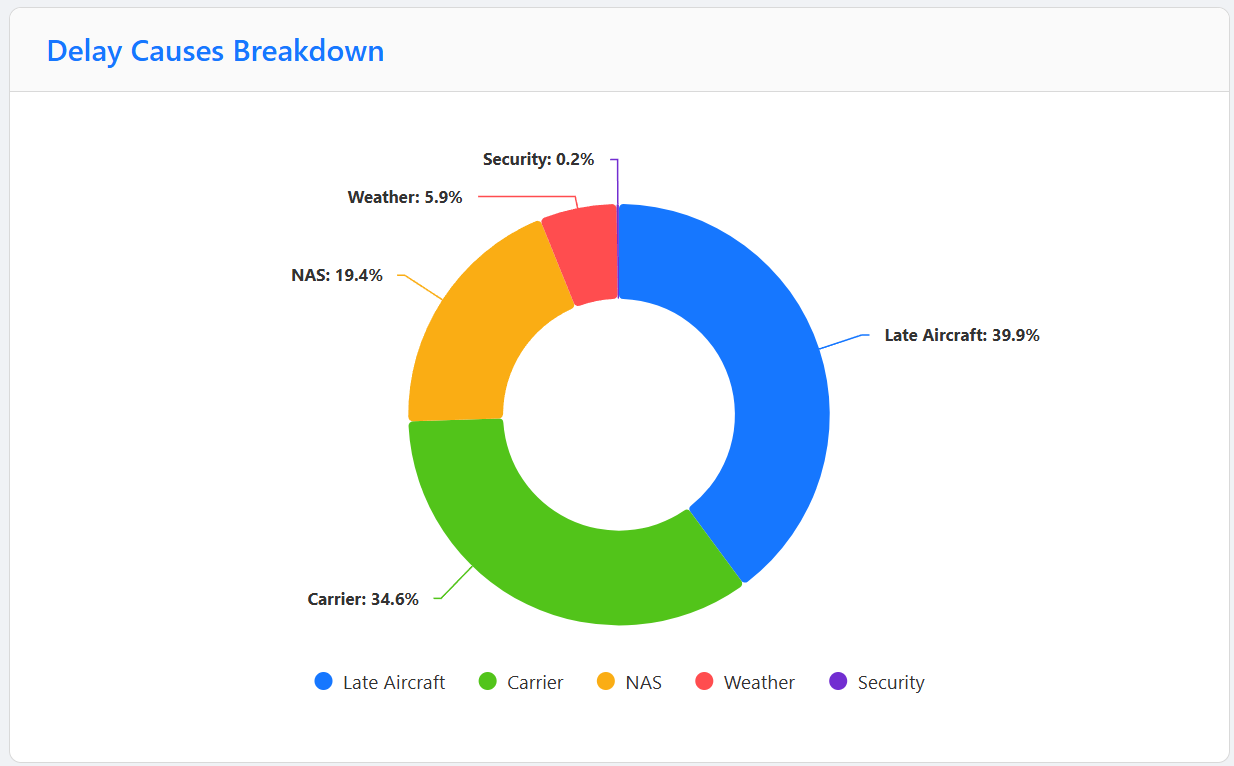
\includegraphics[width=0.9\textwidth]{figures/Bigdata_DelayCauses_FeatureImportance.png}
    \caption{Delay Causes Breakdown and ML Feature Importance Analysis}
    \label{fig:delay_causes}
\end{figure}

\textbf{Late Aircraft Delay (39.9\%):} The largest contributor to delays, accounting for nearly 40\% of total delay minutes. This category represents cascading delays where a late-arriving aircraft causes subsequent flight delays. The high percentage indicates that delays propagate through the network, emphasizing the need for buffer time in scheduling and improved turnaround processes.

\textbf{Carrier Delay (34.6\%):} The second-largest factor, representing delays within the airline's control, such as crew issues, aircraft maintenance, fueling, and baggage loading. This substantial proportion suggests opportunities for operational improvements in airline processes and resource management.

\textbf{National Airspace System (NAS) Delay (19.4\%):} Accounts for delays due to air traffic control, airport operations, and heavy traffic volume. This factor highlights infrastructure and capacity constraints within the aviation system.

\textbf{Weather Delay (5.9\%):} Surprisingly, weather-related delays contribute only a small fraction of total delays. This result suggests that while weather can cause severe disruptions, its overall frequency or duration impact is relatively limited compared to operational factors.

\textbf{Security Delay (0.2\%):} Minimal contribution, indicating that security-related disruptions are rare and well-managed in the current aviation system.

\subsection{Feature Importance for Prediction}

The machine learning model's feature importance analysis reveals that:

\begin{itemize}
    \item \textbf{MONTH (74.5\%):} Dominates prediction capability, confirming strong seasonal patterns in delay occurrence
    \item \textbf{CARRIER (25\%):} Airline identity contributes significantly, indicating performance variability across carriers
    \item \textbf{DISTANCE (<5\%):} Flight distance has minimal predictive power, suggesting delays are more influenced by temporal and operational factors than route length
\end{itemize}

These findings indicate that delay prediction models should prioritize temporal features and carrier-specific characteristics over distance-based metrics.

\section{Airport Performance Analysis}

\begin{figure}[h]
    \centering
    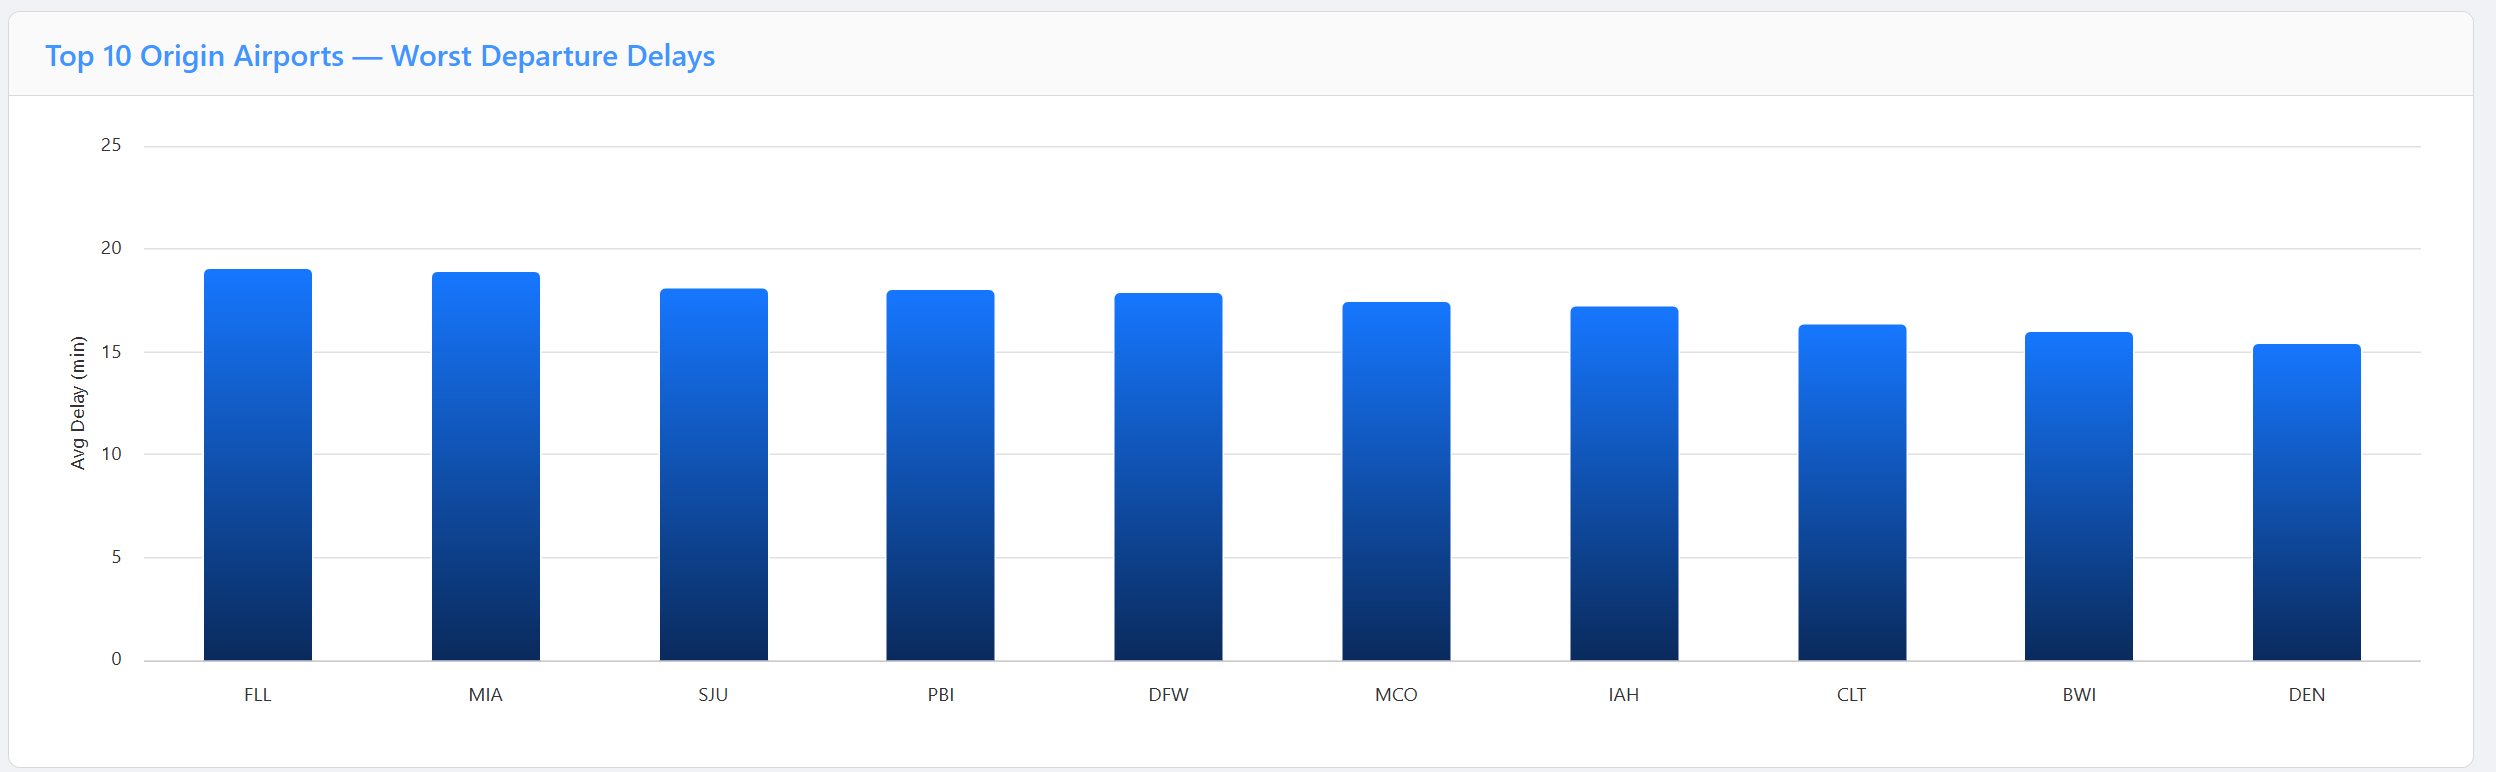
\includegraphics[width=0.9\textwidth]{figures/Bigdata_Top10Airports_Delays.png}
    \caption{Top 10 Origin Airports with Worst Departure Delays}
    \label{fig:airport_delays}
\end{figure}

The analysis identified the top 10 airports with the highest average departure delays, providing insights into geographic and operational bottlenecks in the aviation network.

\subsection{Worst-Performing Airports}

\begin{enumerate}
    \item \textbf{Fort Lauderdale (FLL):} 19.06 minutes average delay
    \item \textbf{Miami (MIA):} 18.89 minutes average delay
    \item \textbf{San Juan (SJU):} 17.93 minutes average delay
    \item \textbf{West Palm Beach (PBI):} 17.72 minutes average delay
    \item \textbf{Dallas/Fort Worth (DFW):} 17.65 minutes average delay
    \item \textbf{Orlando (MCO):} 17.18 minutes average delay
    \item \textbf{Houston (IAH):} 16.98 minutes average delay
    \item \textbf{Charlotte (CLT):} 16.18 minutes average delay
    \item \textbf{Baltimore (BWI):} 15.82 minutes average delay
    \item \textbf{Denver (DEN):} 15.34 minutes average delay
\end{enumerate}

\subsection{Geographic and Operational Insights}

A clear geographic pattern emerges from this analysis. Florida airports (FLL, MIA, PBI, MCO) dominate the top rankings, accounting for 4 of the top 6 positions. This concentration suggests region-specific challenges, potentially related to:

\begin{itemize}
    \item High traffic volume due to tourism and seasonal travel patterns
    \item Weather patterns specific to the Florida region (afternoon thunderstorms)
    \item Airport infrastructure capacity constraints
    \item Hub operations and connecting flight complexities
\end{itemize}

Major hub airports (DFW, IAH, DEN, CLT) also appear in the list, reflecting the operational complexity of coordinating high volumes of connecting flights and the cascading effect of delays in hub-and-spoke networks.

\section{Temporal Delay Patterns}

\begin{figure}[h]
    \centering
    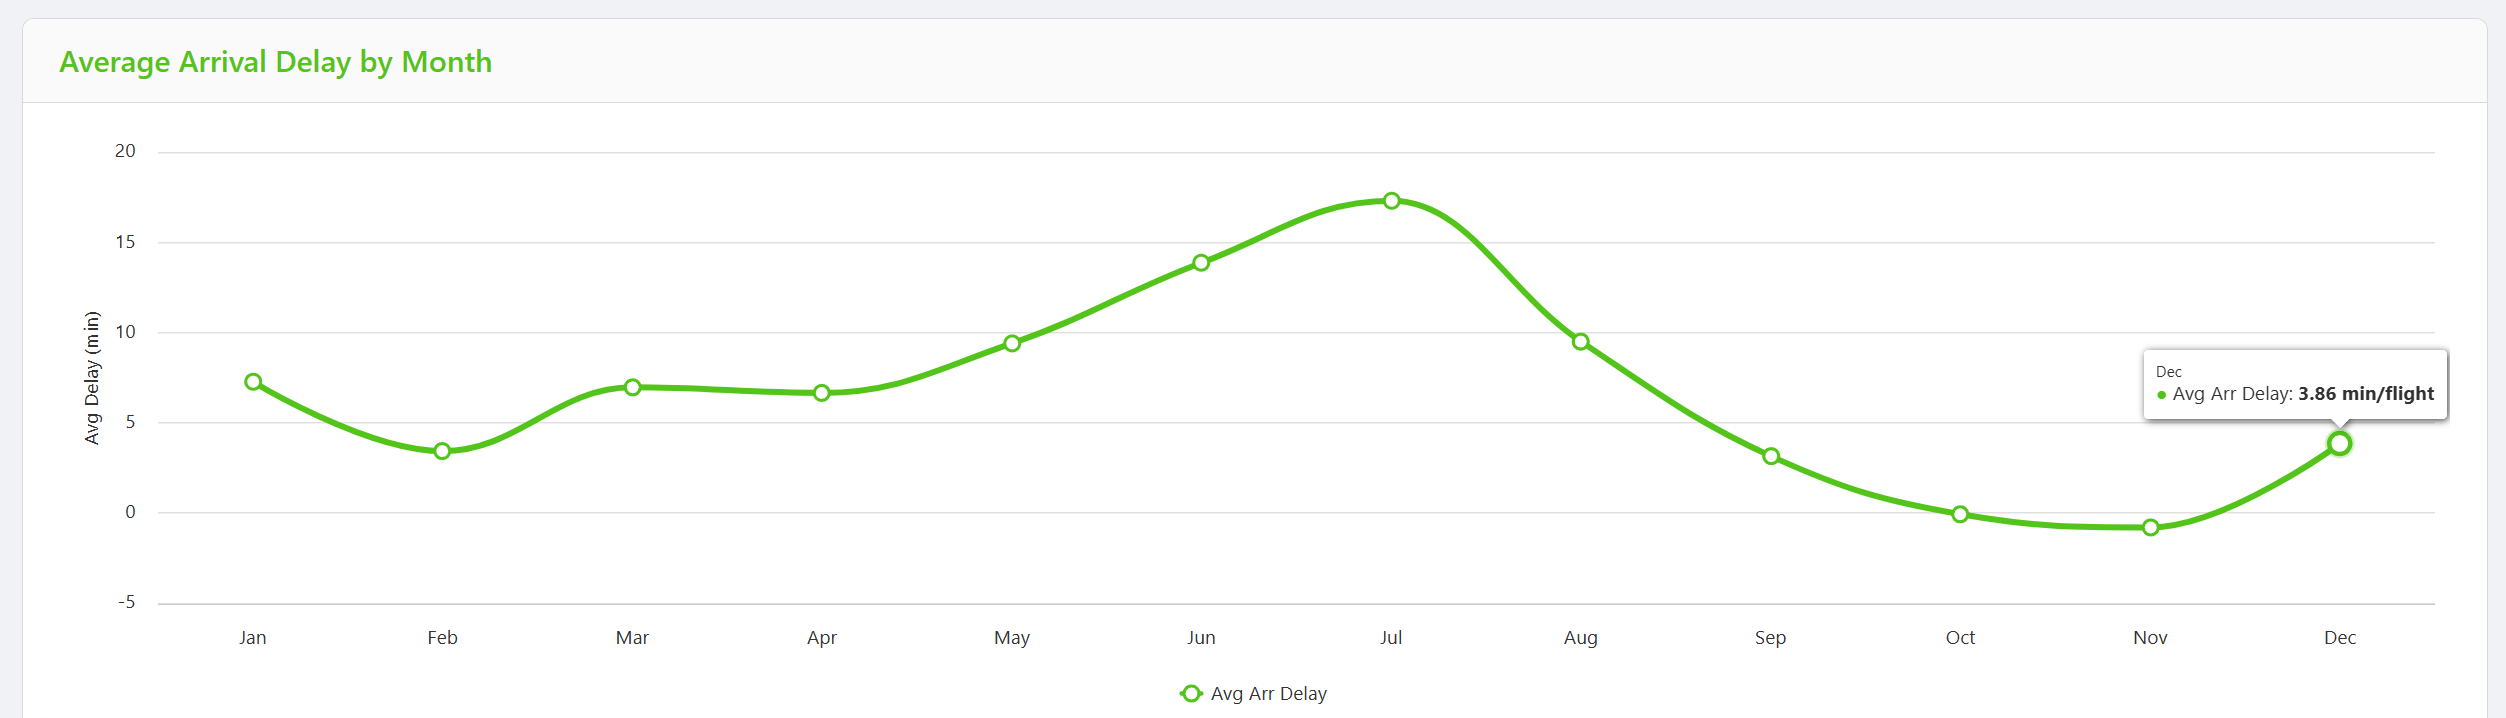
\includegraphics[width=0.9\textwidth]{figures/Bigdata_MonthlyDelays_Trend.png}
    \caption{Average Arrival Delay by Month - Seasonal Trend Analysis}
    \label{fig:monthly_delays}
\end{figure}

The temporal analysis reveals clear seasonal patterns in flight delays, with significant variation across different months of the year.

\subsection{Seasonal Delay Trends}

\textbf{Peak Delay Months (June - July):} Delays reach their maximum during the summer months, with July recording approximately 17 minutes average delay. This peak coincides with:
\begin{itemize}
    \item Summer vacation travel surge
    \item Increased air traffic volume
    \item Weather-related disruptions (thunderstorms)
    \item Higher passenger loads and longer turnaround times
\end{itemize}

\textbf{Moderate Delay Periods (January - May):} The first half of the year shows gradually increasing delays, ranging from 7 minutes in January to 14 minutes in June, reflecting the ramp-up to peak travel season.

\textbf{Low Delay Months (September - November):} The fall months experience the lowest delays, with October and November averaging near-zero delays or even slight early arrivals. This period benefits from:
\begin{itemize}
    \item Reduced travel demand post-summer
    \item Favorable weather conditions
    \item Optimized airline operations with lower capacity utilization
\end{itemize}

\textbf{Year-End Recovery (December):} December shows a slight increase in delays (approximately 4 minutes) due to holiday travel, though significantly lower than summer peaks.

\subsection{Operational Recommendations}

Based on these temporal patterns, airlines and airports should consider:

\begin{itemize}
    \item Implementing dynamic scheduling strategies with increased buffer times during peak months
    \item Allocating additional resources (staff, gates, aircraft) during June-August
    \item Leveraging the low-delay fall period for maintenance and training activities
    \item Developing predictive models that incorporate monthly seasonality as a primary feature
\end{itemize}

\section{Summary of Key Findings}

The comprehensive analysis of 18 million flight records revealed several critical insights:

\begin{enumerate}
    \item \textbf{Predictive Performance:} Machine learning models can achieve 79.46\% accuracy in delay prediction using temporal and carrier features
    \item \textbf{Delay Propagation:} Late aircraft delays (39.9\%) dominate the delay ecosystem, indicating cascading effects throughout the network
    \item \textbf{Operational Control:} Combined carrier and late aircraft delays account for 74.5\% of total delays, suggesting most delays are within the system's control
    \item \textbf{Geographic Concentration:} Florida airports exhibit consistently higher delays, requiring region-specific interventions
    \item \textbf{Seasonal Variability:} Strong monthly patterns exist, with summer experiencing 2-3x higher delays than fall months
    \item \textbf{Feature Dominance:} Temporal factors (month) are 3x more predictive than carrier identity and significantly more important than distance
\end{enumerate}

These findings provide actionable insights for airlines, airport authorities, and aviation regulators to optimize operations, improve scheduling strategies, and enhance passenger experience through data-driven decision-making.





% Chapter 5: CHALLENGES AND SOLUTIONS
\chapter{CHALLENGES AND SOLUTIONS}

\section{Loading Big Data is too slow}

\subsection{Problem}

When loading the 3.4GB CSV file, the system is very slow. It waits for more than 2 minutes and sometimes has memory errors.

\subsection{Cause}

Used \texttt{inferSchema=True}. This means the computer must scan many rows to guess the data type. This is very slow for big data.

\subsection{Solution}

\noindent\textbf{Explicit Schema:} Writing the data structure ourselves. Telling the computer exactly what is in each column.

\noindent\textbf{Result:} The computer does not need to guess anymore. Loading time is now only 13 seconds (10 times faster than before).

\noindent\textbf{Column Pruning:} Only pick 14 important columns from 49. This saves RAM memory.

\section{Machine Learning is too heavy}

\subsection{Problem}

Training a Decision Tree model with 17.7 million rows on one computer is too slow and almost impossible.

\subsection{Cause}

The algorithm must scan all data many times to find the best way to group it.

\subsection{Solution}

\noindent\textbf{Smart Sampling:} Only use 5\% of the data for training. Using a "random seed" to make it reliable. This makes the training very fast (less than 30 seconds).

\noindent\textbf{Feature Importance:} After training, finding that MONTH is the most important factor (77.6\%). This helps understand why flights are late.

\section{Real-time Dashboard}

\subsection{Problem}

The website needs to show the progress clearly. But the system logs from the computer are very messy and hard to read.

\subsection{Cause}

Many messages from the computer are not useful (like "Warning" or "Info").

\subsection{Solution}

\noindent\textbf{Structural Logging:} We changed the computer logs to use clear words like \texttt{[PHASE X]} and \texttt{[Task X]}.

\noindent\textbf{Faster Reading:} The website uses "Regex" to find the important words and time. Now, the progress bar moves correctly and shows how many seconds each step takes.


% References
\begin{thebibliography}{99}
\addcontentsline{toc}{chapter}{References}

\bibitem{spark2016}
Apache Software Foundation, ``Apache Spark: Lightning-fast unified analytics engine,'' 2016. [Online]. Available: https://spark.apache.org/

\bibitem{nextjs2024}
Vercel, ``Next.js: The React Framework for the Web,'' 2024. [Online]. Available: https://nextjs.org/

\bibitem{docker2024}
Docker Inc., ``Docker: Accelerated Container Application Development,'' 2024. [Online]. Available: https://www.docker.com/

\bibitem{hadoop2024}
Apache Software Foundation, ``Apache Hadoop: Distributed Storage and Processing,'' 2024. [Online]. Available: https://hadoop.apache.org/

\bibitem{huggingface2024}
Hugging Face, ``flight\_delay Dataset,'' 2024. [Online]. Available: https://huggingface.co/datasets/

\bibitem{react2024}
Meta Platforms, ``React: A JavaScript library for building user interfaces,'' 2024. [Online]. Available: https://react.dev/

\bibitem{highcharts2024}
Highsoft AS, ``Highcharts: Interactive JavaScript charts for web pages,'' 2024. [Online]. Available: https://www.highcharts.com/

\bibitem{antd2024}
Ant Design Team, ``Ant Design: A UI Design Language and React UI library,'' 2024. [Online]. Available: https://ant.design/

\end{thebibliography}

% Appendices 
\appendix

\chapter{Glossary}

\begin{description}
    \item[Big Data] Extremely large datasets that require specialized processing techniques
    \item[Docker Container] A lightweight, standalone executable package that includes everything needed to run software
    \item[HDFS] Hadoop Distributed File System - a distributed file system designed to run on commodity hardware
    \item[Machine Learning] A subset of artificial intelligence that enables systems to learn from data
    \item[Pipeline] A series of data processing steps executed in sequence
    \item[Spark] An open-source unified analytics engine for large-scale data processing
    \item[SSE] Server-Sent Events - a technology for pushing updates from server to client
\end{description}

\end{document}
